\documentclass[11pt]{beamer}
\usetheme{CambridgeUS}
\usepackage[utf8]{inputenc}
\usepackage{amsmath}
\usepackage{amsfonts}
\usepackage{amssymb}
\usepackage{graphicx}

\setbeamercovered{transparent} %gray-out for pause


\usepackage{listings}
\usepackage{pifont}
\usepackage{ulem}

\definecolor{Black}{RGB}{0,0,0}
\definecolor{Red}{RGB}{255,0,0}
% colors
\definecolor{Orange}{rgb}{1,0.5,0}
\definecolor{Blue}{RGB}{0,0,255}
\definecolor{OrangeRed}{RGB}{255,69,0}
\definecolor{LightGreen}{RGB}{11,83,69}
\definecolor{DarkYellow}{RGB}{160,64,0}
\definecolor{AntiqueBrass}{rgb}{0.8, 0.58, 0.46}
\definecolor{NiceBlue}{RGB}{11, 102, 163}
\definecolor{NiceRed}{RGB}{160, 64, 0}
\definecolor{Grey}{RGB}{128,128,128}
\definecolor{SlightRed}{RGB}{249,38,114}
\definecolor{SlightPink}{RGB}{155, 89, 182}

\newcommand{\hgb}[1]{{\color{Blue}{#1}}}
\newcommand{\hgr}[1]{{\color{OrangeRed}{#1}}}
\newcommand{\hgd}[1]{{\color{Red}{#1}}}
\newcommand{\head}[2]{{\textbf{#2}, #1}}

% syntax highlighting
\usepackage{textcomp} % other glyphs needed for upquote in listings below
\lstdefinelanguage{HorseIR}
{ basicstyle=\footnotesize\ttfamily,
  commentstyle=\color{Grey}\rmfamily\itshape,
  keywordstyle=\color{SlightPink},
  keywordstyle=[2]\color{NiceBlue},
  keywordstyle=[3]\color{NiceRed},
  keywordstyle=[4]\color{SlightRed},
  % list of keywords
  morekeywords={
  module,
  def,
  import
  },
  keywords=[2]{
  @table,
  @sum,
  @gt,
  @load_table,
  @column_value,
  @and,
  @compress,
  @enum,
  @list,
  @group,
  @values,
  @each_right,
  @raze,
  @compute_discount
  },
  keywords=[3]{
  table,
  sym,
  list,
  i64,
  f64,
  bool,
  },
  keywords=[4]{
  return,
  check_cast
  },
  sensitive=false, % keywords are not case-sensitive
  morecomment=[l]{//}, % l is for line comment
  morecomment=[s]{/*}{*/}, % s is for start and end delimiter
  morestring=[b]", % defines that strings are enclosed in double quotes
  upquote=true % ensures that backtick displays correctly
}


\author{Hanfeng Chen}
\title{
  {\color{Black}{Improving Database Performance on Modern Hardware}}
}
%\subtitle{{\color{Black}{(Combining array languages and in-memory databases)}}}
%\setbeamercovered{transparent} 
%\setbeamertemplate{navigation symbols}{} 
%\logo{} 
%\institute{McGill University}
\date{2018.04.11}
%\subject{} 
\begin{document}

\begin{frame}
\titlepage
\end{frame}


%\section*{Outline}
%\begin{frame}
%\tableofcontents
%\end{frame}

\AtBeginSection[]
  {
     \begin{frame}<beamer>
     \frametitle{Outline}
     \tableofcontents[currentsection]
     \end{frame}
  }

\section{Introduction}
\begin{frame}{Introduction}

The goal of SQL query processing

\pause
\begin{itemize}
\item Performance: \hgr{low} response time and \hgb{high} throughputs
\end{itemize}

\pause
How to achieve the goal

\begin{itemize}
\pause
\item Implement a fast interpreter (Conventional approach)
\pause
\item Compile SQL to relatively low-level languages, such as C++/LLVM (Recent decade)
\pause
\item Adopt new hardware devices, such as GPU/FPGA (Latest!)
\end{itemize}
\end{frame}

\begin{frame}{Approach} 
Levels of difficulty 
\begin{itemize}
\item Interpreter \textless\ Compiler+CPU \textless\ Compiler+GPU
\end{itemize} 
\pause
State-of-the-art approach
\begin{itemize} 
\item A high-level abstraction for generating \hgb{robust} and
\hgr{efficient} code
\item Platform-specific strategies for optimizing code
\item Relatively low compilation time compared with execution time
\end{itemize} 
\end{frame}

\begin{frame}{Topics} 
Topics in this presentation
\begin{enumerate}
\item Compiling queries to LLVM with/without adaptive execution
\item Generating efficient code for modern hardware from a vector algebra 
\end{enumerate}
\end{frame}

\begin{frame}{Topics} 
\textbf{I:} Compiling queries to LLVM with/without adaptive execution
\begin{enumerate}
\item \head{Thomas}{Neumann},
      ``\uline{Efficiently compiling efficient query plans for modern hardware}",
      PVLDB, 2011, vol. 4, no. 9, pp. 539--550
\item \head{Andre}{Kohn}, Viktor Leis, Thomas Neumann,
      ``\uline{Adaptive Execution of Compiled Queries}", 2018, appear soon.
\end{enumerate} 
\pause
\textbf{II:} Generating efficient code for modern hardware from a vector algebra 
\begin{enumerate} 
\item \head{Holger}{Pirk}, Oscar Moll, Matei Zaharia, Sam Madden,
      ``\uline{Voodoo - A Vector Algebra for Portable Database Performance on Modern Hardware}",
      PVLDB, 2016, vol. 9, no. 14, pp. 1707--1718 
\end{enumerate}
\end{frame}


%\section{Related Work}
%\input{src/related}

\section{Part I: Compiled Queries}
\begin{frame}{HyPer}
The overview of HyPer
\begin{itemize}
\item HyPer targets main-memory database
\item HyPer compiles SQL to LLVM
\item HyPer mixes LLVM and C++ before generating machine code
\end{itemize}
\begin{figure}[htb]
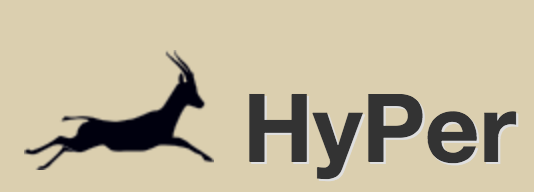
\includegraphics[width=0.4\textwidth]{fig/hyper-logo.png}
\end{figure}
\end{frame}

\begin{frame}{HyPer: An Example}
A simple example
\begin{figure}[htb]
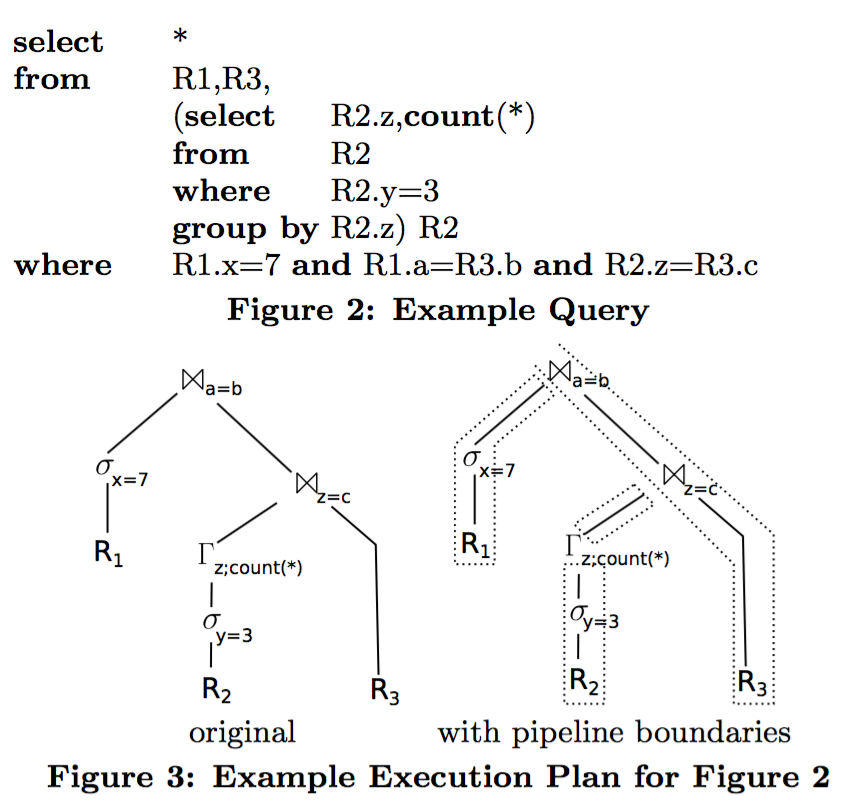
\includegraphics[width=0.5\textwidth]{fig/hyper-fig2.png}
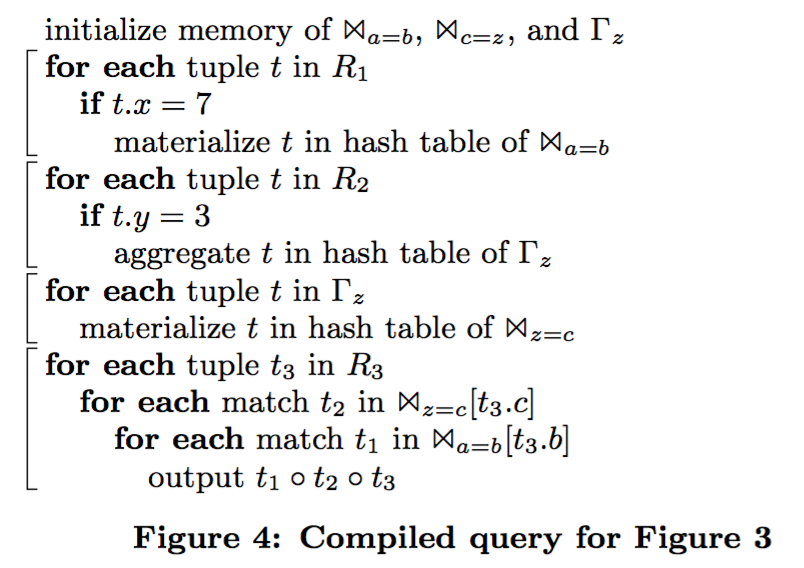
\includegraphics[width=0.5\textwidth]{fig/hyper-fig4.png}
\end{figure}
\end{frame}

\begin{frame}{HyPer: Evaluation}
Show the OLAP part (online analytic processing)
\begin{figure}[htb]
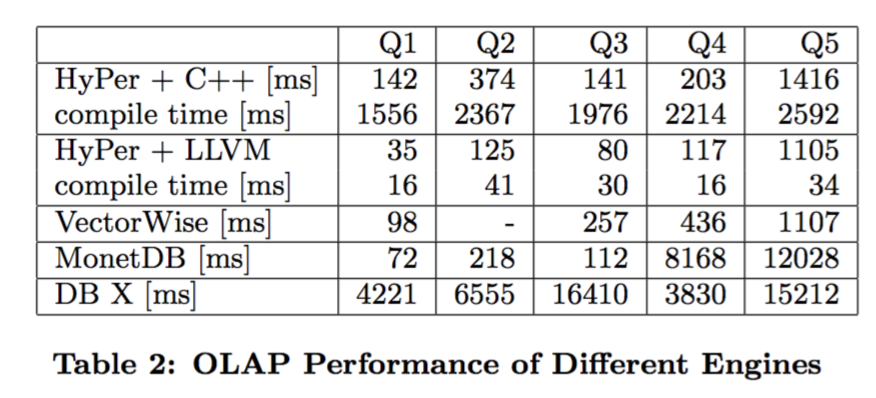
\includegraphics[width=0.6\textwidth]{fig/hyper-table2.png}
\end{figure}
\begin{itemize}
\item TPC-H benchmarks: Q1-5
\item HyPer + LLVM has significantly low compile time
\end{itemize}
\end{frame}

% Start adaptive execution

\begin{frame}{HyPer: Adaptive Execution}
Adaptive execution is necessary, when
\begin{itemize}
\item processing many complex but quick queries, because compiling complex
      queries usually may take hundreds of milliseconds.
\end{itemize}
\pause
Possible applications
\begin{itemize}
\item Streaming/real-time queries
\end{itemize}
\pause
Implementation
\begin{itemize}
\item Kohn et al. implemented a fast bytecode interpreter for LLVM to save the costly compile time
\end{itemize}
\end{frame}

\begin{frame}{Adaptive Execution}
Architecture of compilation-based query engines
\begin{figure}[htb]
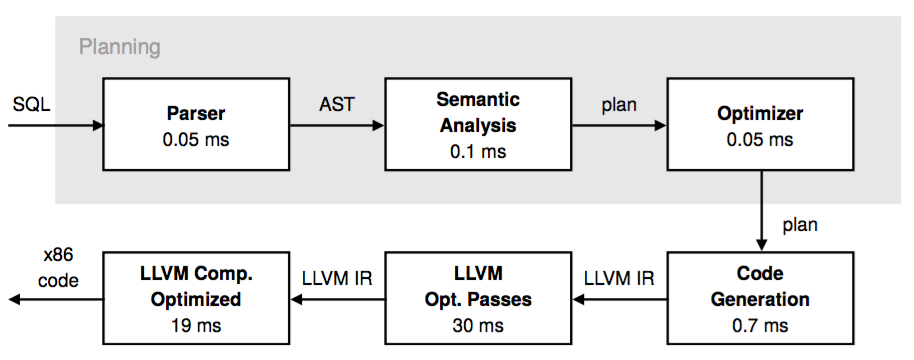
\includegraphics[width=0.6\textwidth]{fig/adaptive-fig1.png}
\end{figure}
\begin{itemize}
\item LLVM optimizations dominate the whole pipeline (very expensive!)
\end{itemize}
\end{frame}

\begin{frame}{Adaptive Execution}
Three modes: 1) LLVM Opt. 2) LLVM Unopt. and 3) Byte Code Compiler
\begin{figure}[htb]
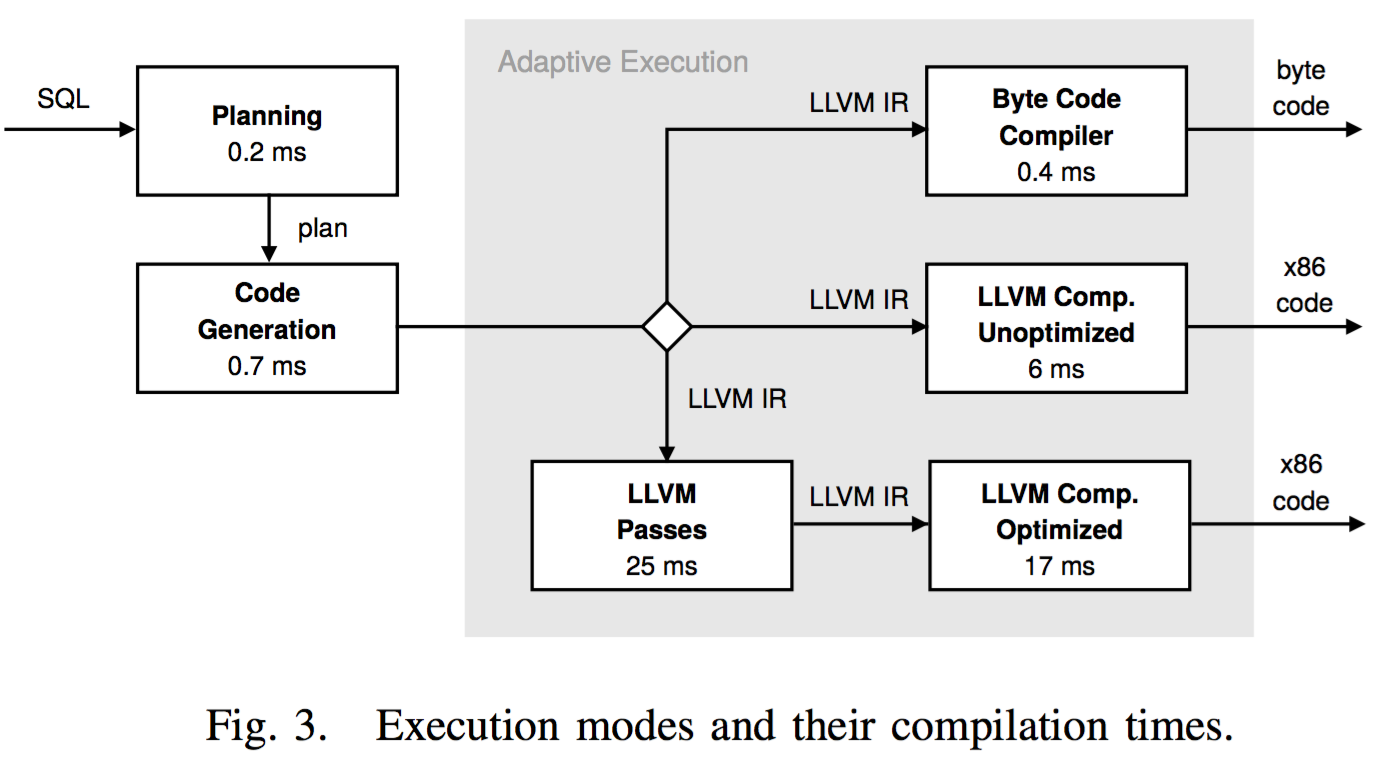
\includegraphics[width=0.8\textwidth]{fig/adaptive-fig3.png}
\end{figure} 
\end{frame}

\begin{frame}{Execution Modes}
The challenge question is how to switch between three modes seamlessly.
\begin{itemize}
\item Split an query into smaller units, called \hgb{morsels}
\item Switch between morsels which are the \hgr{smallest} units
\end{itemize}
\end{frame}

\begin{frame}{Execution Modes}
Switch on-the-fly
\begin{figure}[htb]
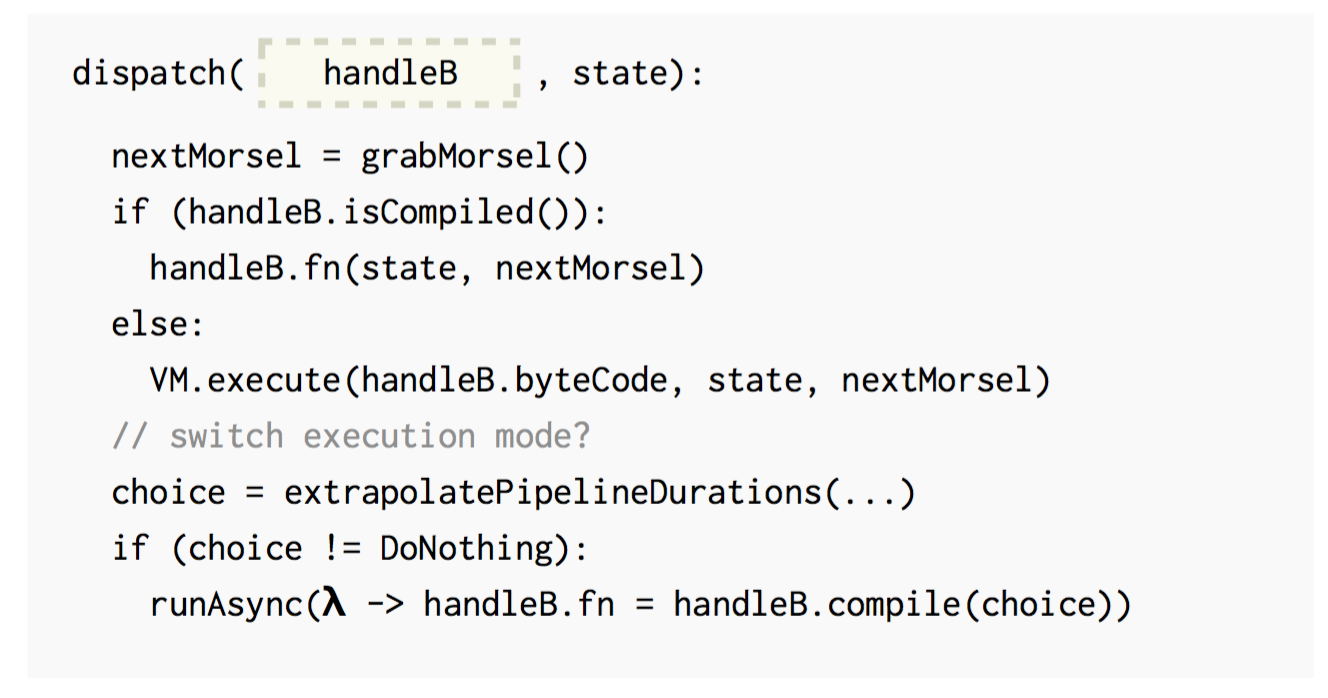
\includegraphics[width=0.8\textwidth]{fig/adaptive-fig5.png}
\end{figure} 
\end{frame}

\begin{frame}{Virtual Machine}
Overview
\begin{itemize}
\item A register-based machine
\item Fixed-length, statically typed
\end{itemize}
Example: from LLVM to VM code
\begin{figure}[htb]
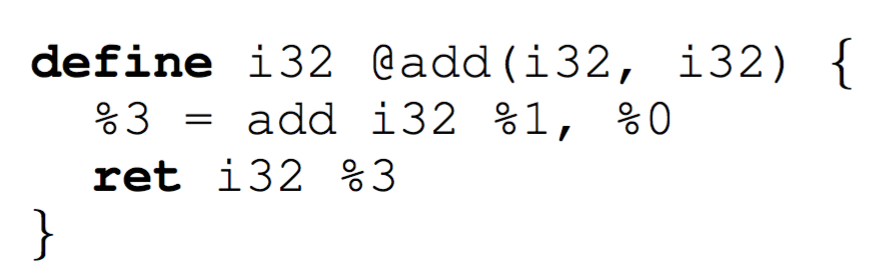
\includegraphics[width=0.4\textwidth]{fig/adaptive-code1.png}
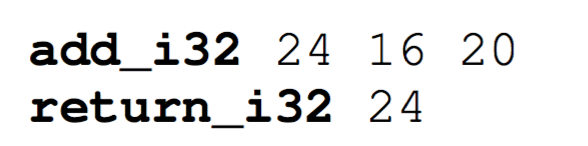
\includegraphics[width=0.28\textwidth]{fig/adaptive-code2.png}
\end{figure} 
\pause
\large{Conventional design!}
\end{frame}

\begin{frame}{Optimization}
Linear-Time Liveness Computation
\begin{itemize}
\item Traditional method has O($n^2$) which is not tolerable
\item New method needs basic blocks in reversed postorder and dominator trees
\end{itemize}
\pause
\hgr{Questions}
\begin{itemize}
\item An iteration-based fix-point solver may be faster
\item Computing dominator trees directly requires O($n^2$)
\end{itemize}
\end{frame}

\begin{frame}{Evaluation}
Show TPC-H results
\begin{figure}[htb]
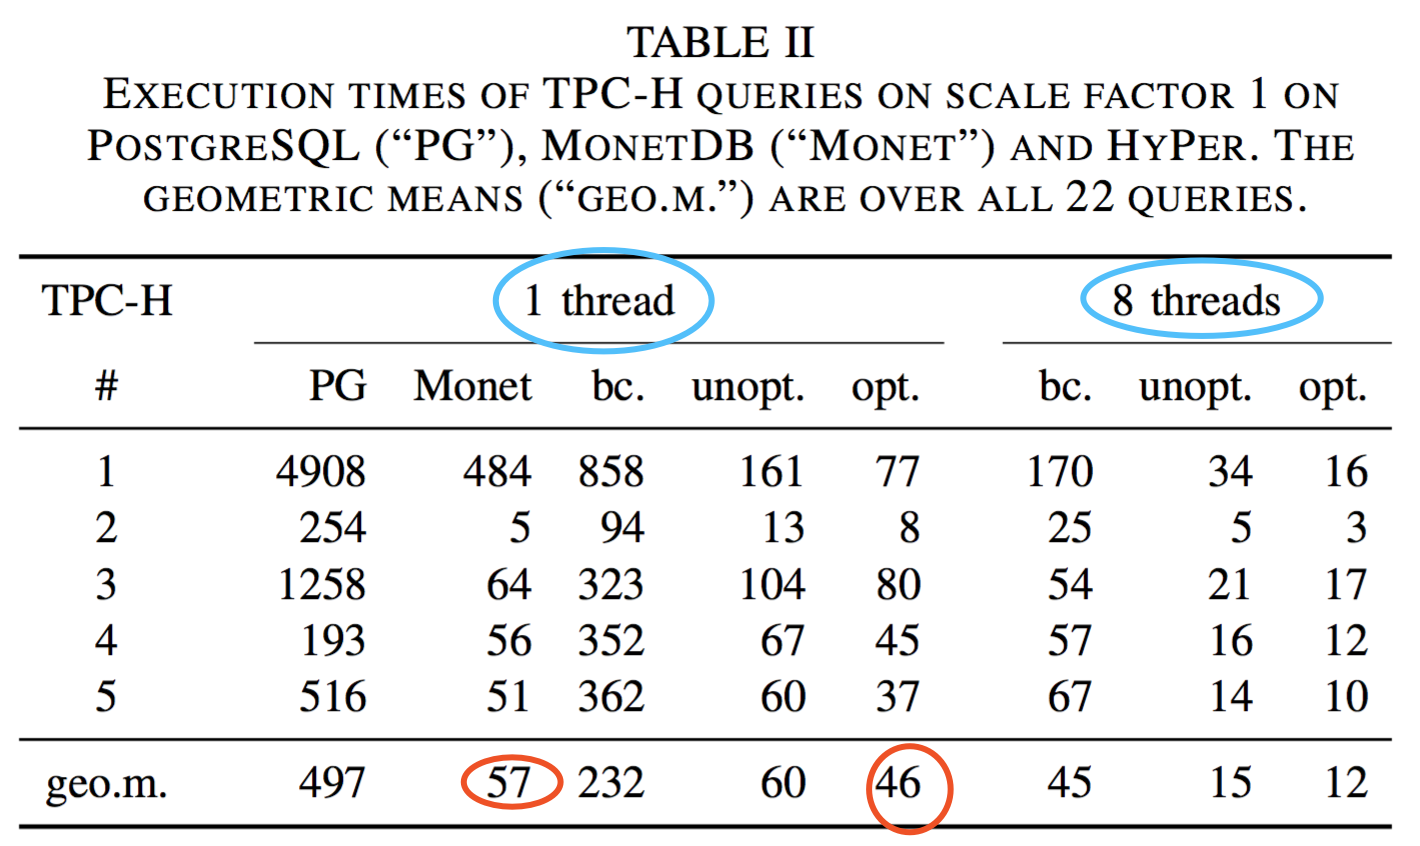
\includegraphics[width=0.6\textwidth]{fig/adaptive-table2.png}
\end{figure} 
\begin{itemize}
\item In 1 thread, opt. is 19\% faster than MonetDB
\item The performance of byte code has been improved a lot with 8 threads.
\end{itemize}
\end{frame}

\begin{frame}{Summary}
Brief summary
\begin{itemize}
\item Interpretation and compilation are both important
\item Adaptive execution with three modes
\item Flexible capability of processing data ranging from 10MB to 30GB
\end{itemize}
\pause
What we learn
\begin{itemize}
\item Switching between different modes may benefit the performance of overall system
\item HorseIR naturally has \texttt{morsels} which are primitive functions
\end{itemize}
\end{frame}


% Voodoo, HorseIR
\section{Part II: Vector Algebra}
\begin{frame}{Voodoo: A Vector Algebra for Database Operations}
The overview of Voodoo
\begin{itemize}
\item A declarative intermediate algebra targeting in-memory databases
\item Abstracts hardware details
\item Vector oriented
\item Easy to generate low-level code (e.g. C/OpenCL)
\item Easy to be optimized (e.g. vectorization)
\end{itemize}
\end{frame}

\begin{frame}{Voodoo}
\begin{figure}[htb]
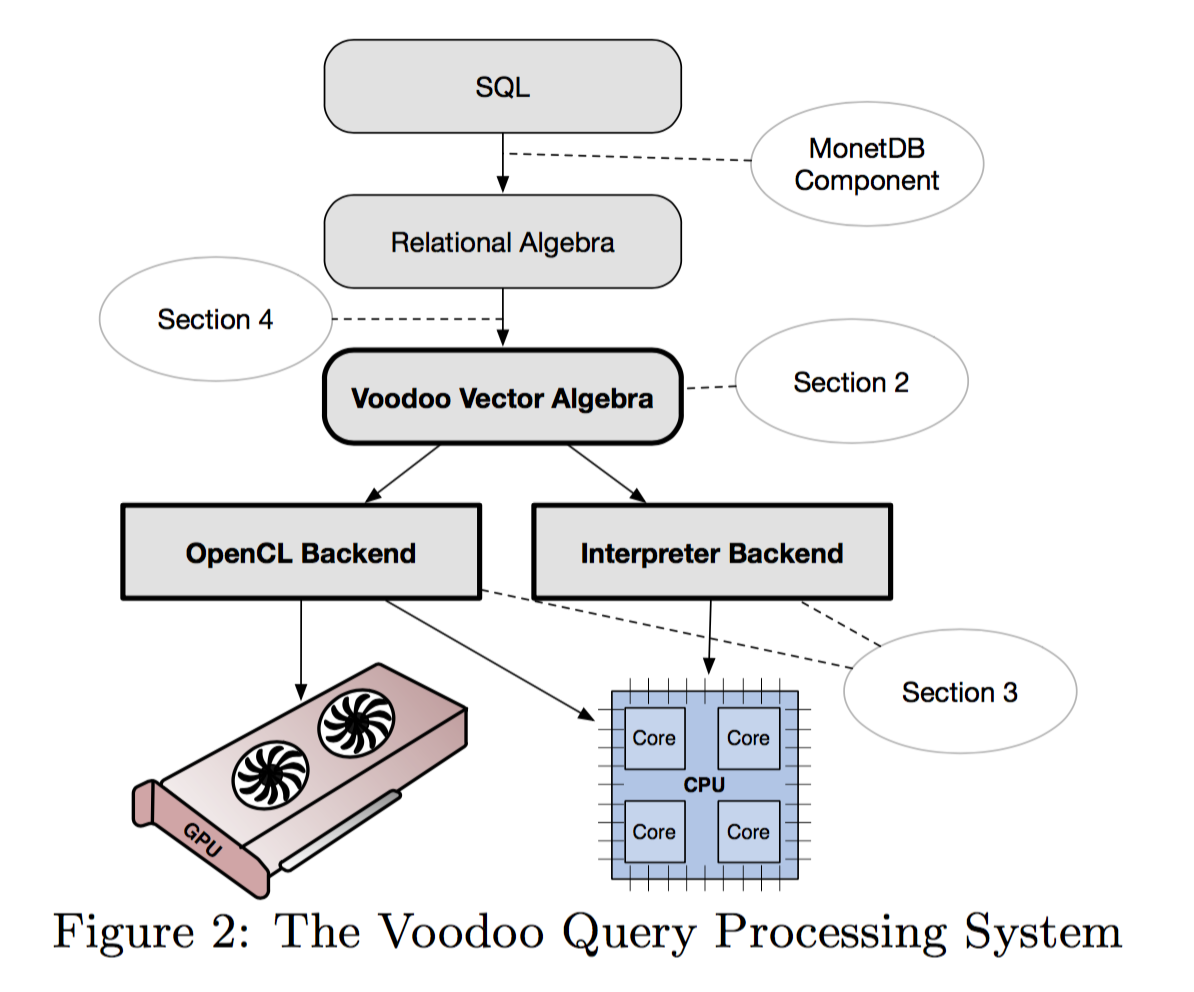
\includegraphics[width=0.85\textwidth]{fig/voodoo-fig2.png}
\end{figure}
\end{frame}

\begin{frame}[fragile]{Voodoo: Example}
Example 1: Multithreaded hierarchical aggregation in Voodoo

\begin{lstlisting}[basicstyle=\footnotesize]
1 input        := Load("input")
2 ids          := Range(input)
3 partitionSize:= Constant(1024)
4 positionIDs  := Divide(ids, partitionSize)
5 positions    := Partition(partitionIDs)
6 inputWPart   := Zip(input, partitionIDs)
7 partInput    := Scatter(inputWPart, positions)
8 pSum         := FoldSum(partInput.val,partInput.partition)
9 totalSum     := FoldSum(pSum)
\end{lstlisting}
\begin{itemize}
\item Line 3 and 4 create a vector that maps each tuple to a partition
\item Line 7 partitions the input according to positions
\item Line 8 and 9 performs aggregations on segments and the entire input respectively
\end{itemize}
\end{frame}

\begin{frame}[fragile]{Voodoo: Example}
Example 2: Adapt to SIMD in Voodoo, need to change
\begin{lstlisting}[basicstyle=\small]
line 3: laneCount    := Constant(2)
line 4: partitionIDs := Modulo(ids, laneCount)
\end{lstlisting}
\end{frame}

%\begin{itemize}
%\item Load: load a vector from persistent storage
%\item Range: generate a vector 1..step..n
%\item Zip: zip two vectors x,y into a new vector $\{(x_i, y_i)\}$
%\item Partition: generate a scatter position vector
%\end{itemize} 

\begin{frame}{Voodoo: Features}
Features
\begin{itemize}
\item Structured vectors (data): one-dimensional arrays
\item Controlled folding (a novel method): folding with a boolean mask
\item Operators in four categories: a rich set of operators
\end{itemize}
\end{frame}

\begin{frame}{Controlled folding}
\begin{figure}[htb]
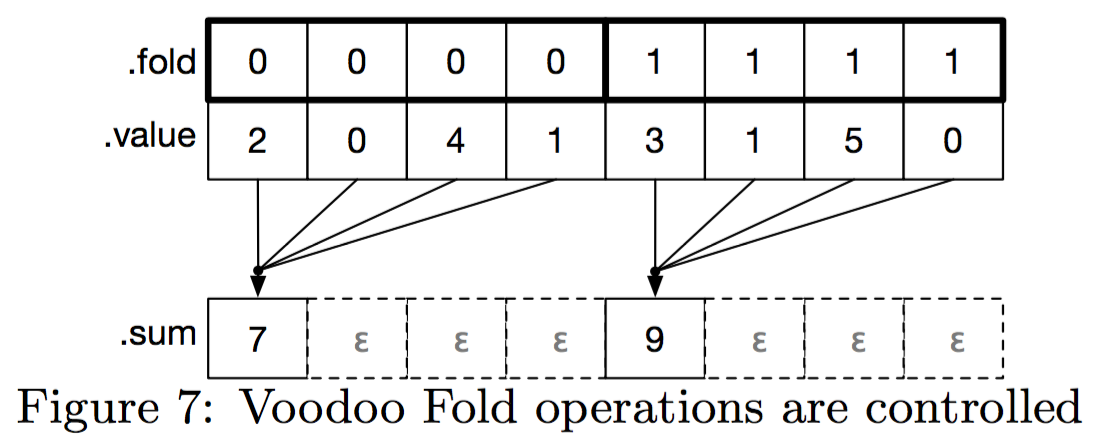
\includegraphics[width=0.7\textwidth]{fig/voodoo-fig7.png}
\end{figure}
\end{frame}

\begin{frame}[fragile]{Controlled folding}
The equivalent code in HorseIR is
\begin{lstlisting}[language=HorseIR, basicstyle=\footnotesize]
t0 = @compress(fold, value)
t1 = @sum(t0)
\end{lstlisting}
When generating code from HorseIR, the idea of controlled folding can be
applied by fusing this adjacent two lines of code.
\end{frame}

\begin{frame}{Voodoo Operators}
\begin{enumerate}
\item Maintenance operations: I/O, such as Load
\item Data-parallel operations: such as logical expressions
\item Fold operations: database specials
\item Shape operations: such as Range
\end{enumerate}

As far as we can see, the design of Voodoo intends to become database-friendly.
\end{frame}

\begin{frame}{OpenCL Back-end}
\begin{figure}[htb]
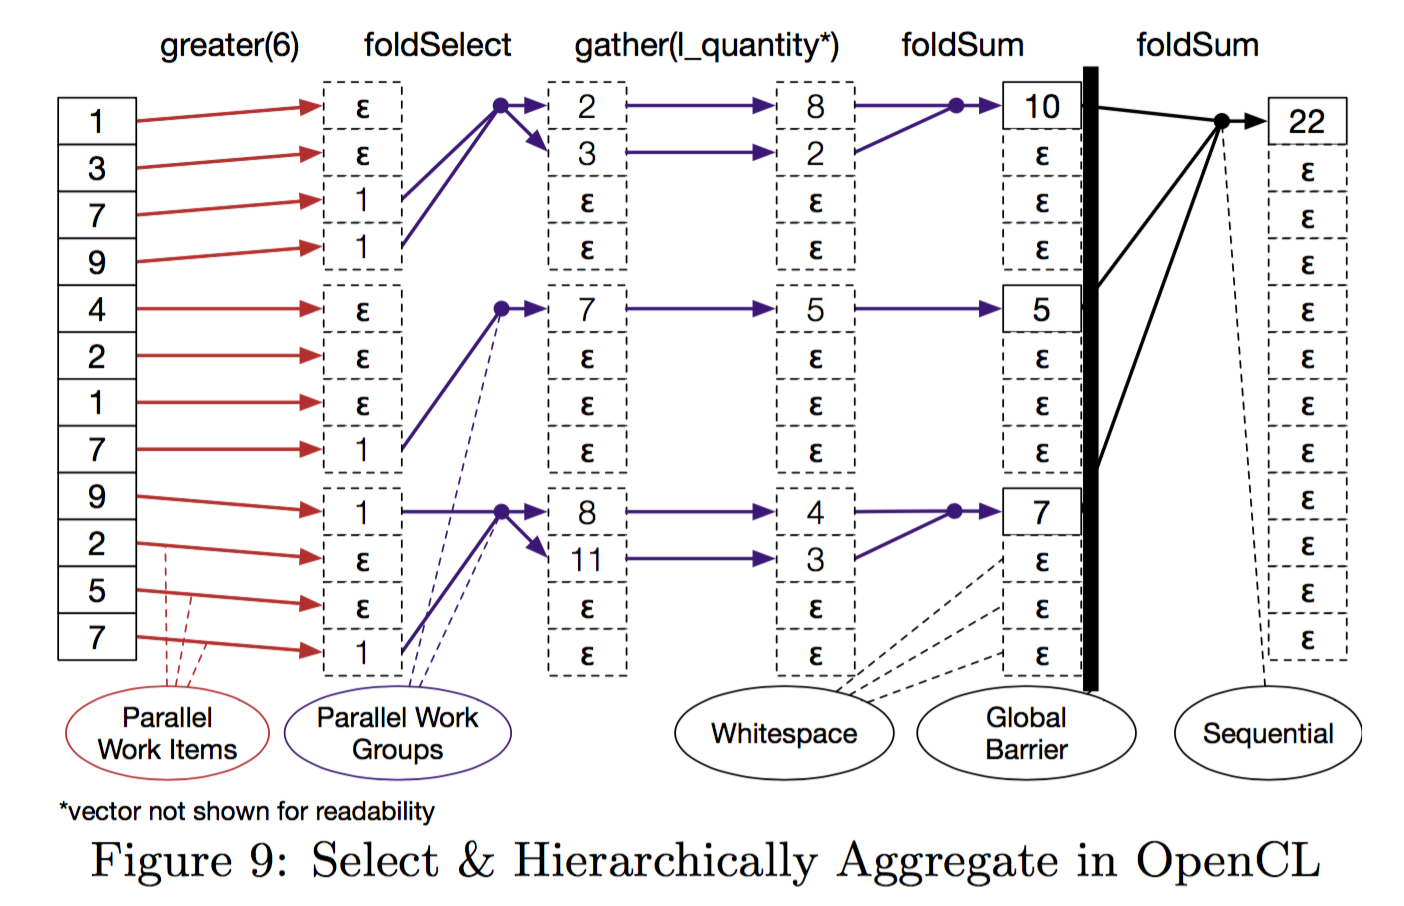
\includegraphics[width=0.8\textwidth]{fig/voodoo-fig9.png}
\end{figure}
\end{frame}

\begin{frame}{Evaluation}
Setup
\begin{itemize}
\item TPC-H benchmarks
\item GPU: MonetDB/Ocelot vs. Voodoo/GPU
\item CPU: HyPeR vs. Voodoo/CPU
\item Only the execution time counted
\end{itemize}
\end{frame}

\begin{frame}{Evaluation: GPU}
\begin{figure}[htb]
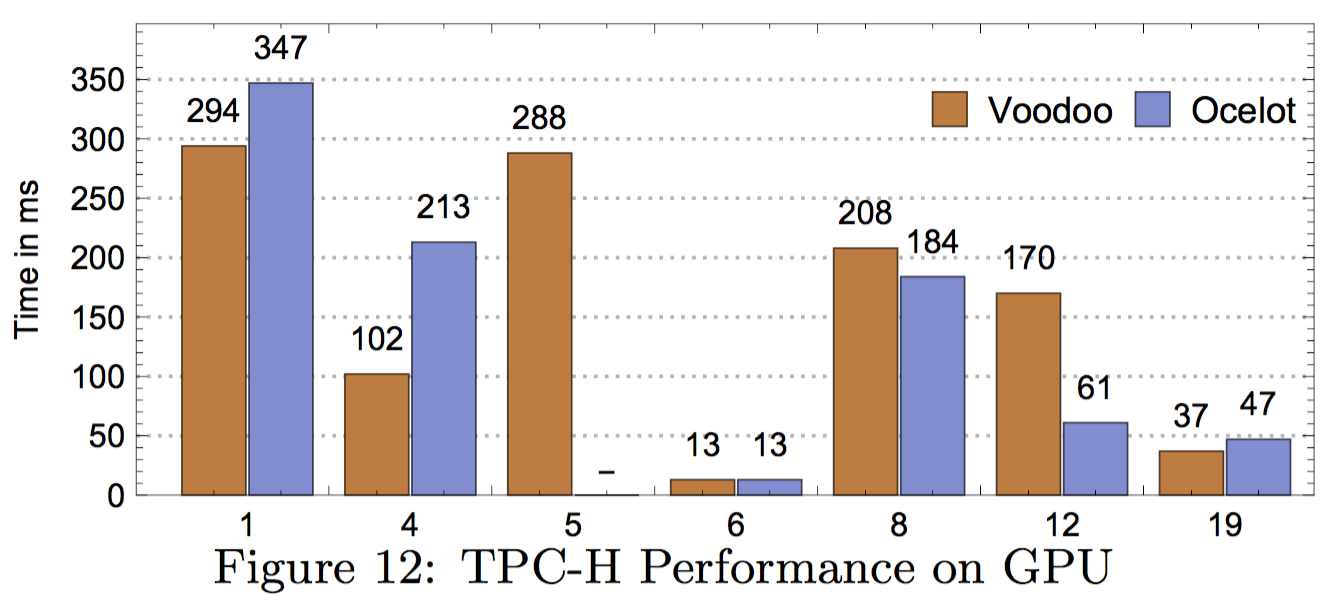
\includegraphics[width=0.8\textwidth]{fig/voodoo-fig12.png}
\end{figure}
\begin{itemize}
\item Voodoo \textgreater\ Ocelot in 3 queries (q1/4/19)
\end{itemize} 
\end{frame}

\begin{frame}{Evaluation: CPU}
\begin{figure}[htb]
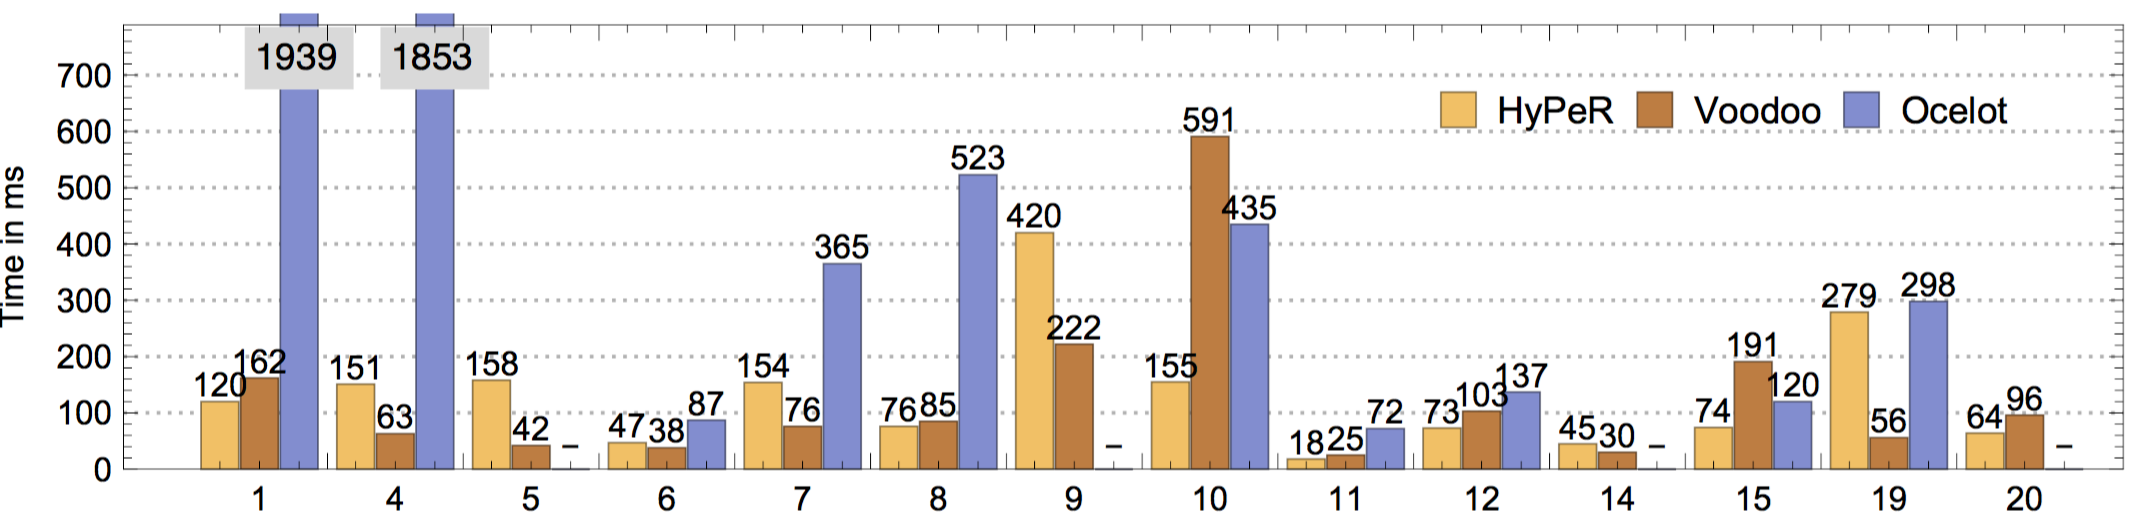
\includegraphics[width=1\textwidth]{fig/voodoo-fig13.png}
\end{figure}
\begin{itemize}
\item HyPeR and Ocelot target CPU and GPU respectively
\item Observation: HyPeR \textgreater Voodoo (7), HyPeR \textless Voodoo (7)
\end{itemize} 
\end{frame}

\begin{frame}{Summary}
Brief summary
\begin{itemize}
\item Voodoo is an intermediate vector algebra
\item The paper presents a novel technique: control vectors
\item Voodoo makes it easy to explore optimizations for different architectures
\end{itemize} 
\pause
However, we can see some restrictions:
\begin{itemize}
\item No support for non-homogeneous data, such as lists
\item No systemic design of operators (build-in functions)
\item Thus, not easy for optimizations on the level of Voodoo
\end{itemize} 
\end{frame}



\section{Conclusion}
\begin{frame}{Conclusions}
Conclusions
\begin{itemize}
\item We need interpretation because sometimes compilation is expensive 
\item We should consider the cost of optimizations at compile time
\item We need a high-level abstraction for supporting various back-ends
\end{itemize}
\end{frame}


% \begin{frame}[t,allowframebreaks]{References}
% \bibliographystyle{amsalpha}
% \bibliography{reference.bib}
% \end{frame}

\end{document}
